\documentclass{beamer}
\usepackage{graphicx}
\usepackage{chancery}
\usepackage{color}
\usepackage{setspace}
\usepackage{ragged2e}
\usepackage{color}

\definecolor{Color1}{rgb}{0.4,1,0.5}
\definecolor{Color2}{rgb}{1,0.35,0.35}
\definecolor{Color3}{rgb}{0.9,1,0.6}
\definecolor{Color4}{rgb}{0.6,0,0}

\begin{document}

\setbeamertemplate{navigation symbols}{\color{white} \insertframenumber/29}
\setcounter{framenumber}{9}
{
\usebackgroundtemplate{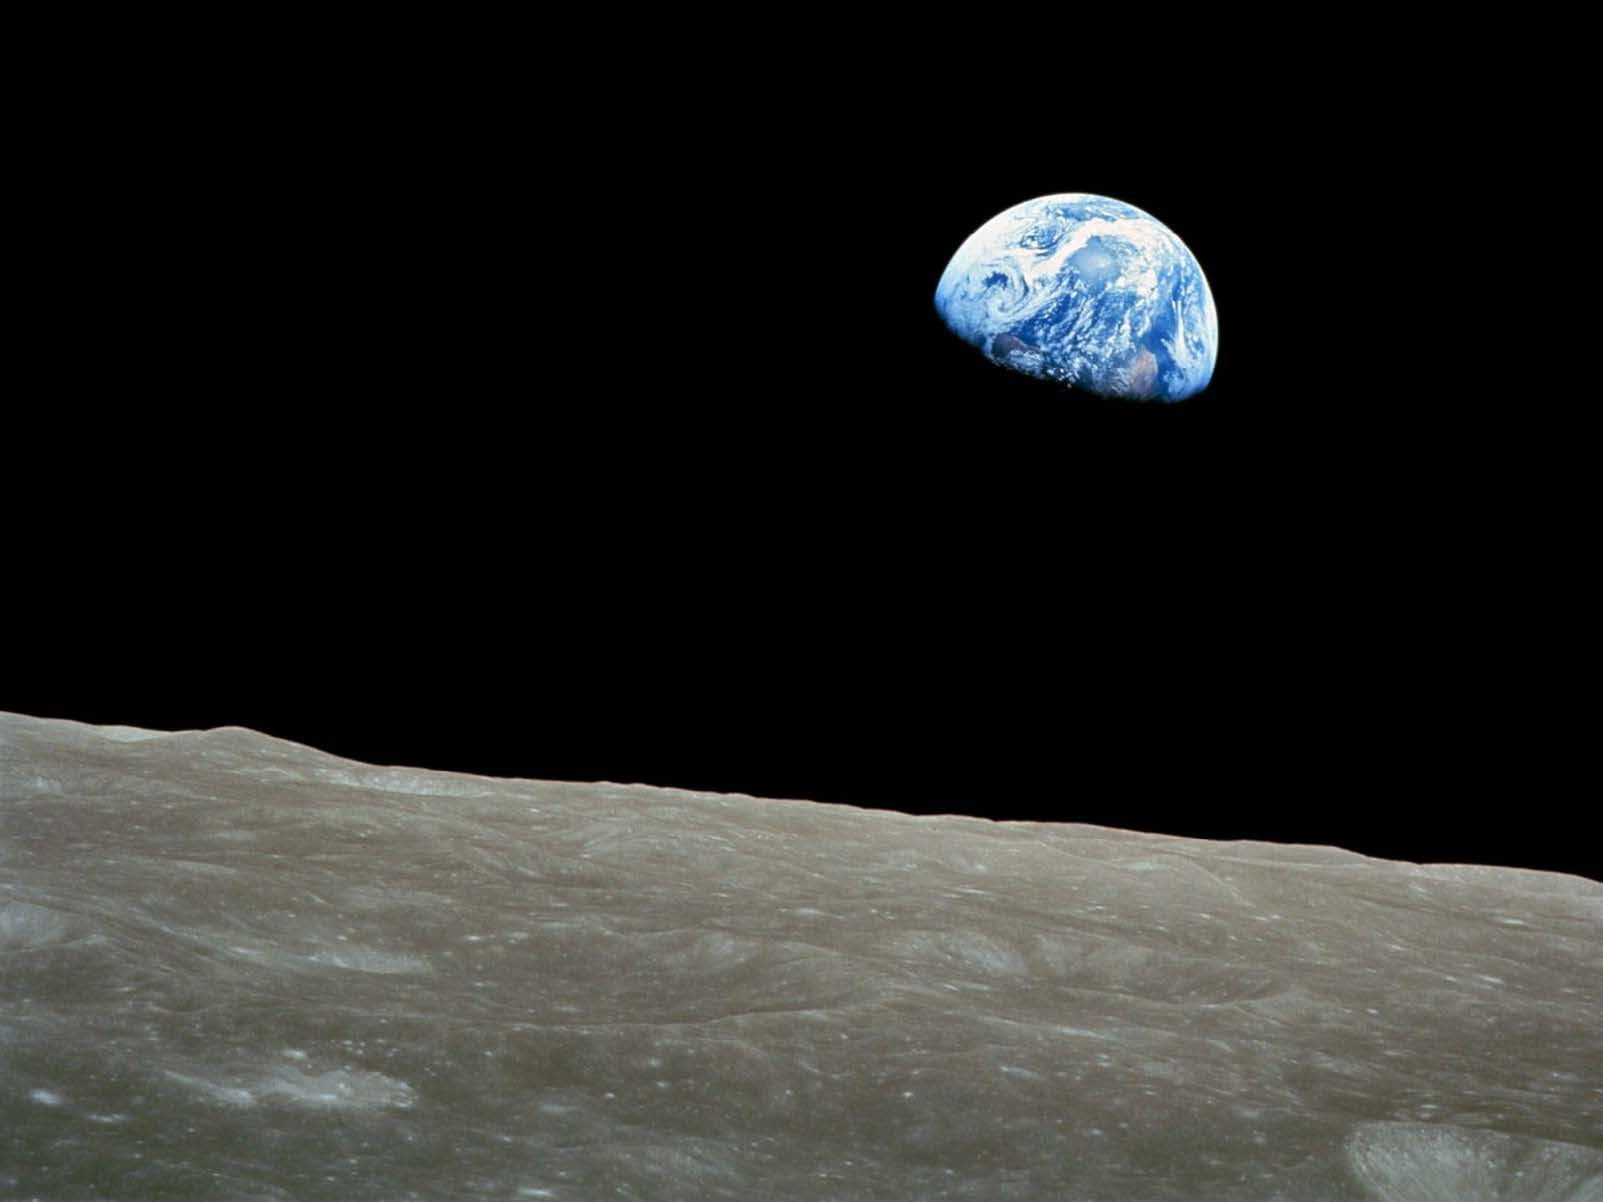
\includegraphics{pic2_10.jpg}}	

\begin{frame}
\pause
\vspace{30pt}
\Huge \color{white}{See things from the other side}
\end{frame}
}

\setcounter{framenumber}{16}
\setbeamercolor{background canvas}{bg=black}
\begin{frame}
\begin{columns}
		
\begin{column}{0.5\linewidth}
\begin{figure}
\includegraphics<1>[width=\linewidth]{pic2_17_1.png}
\includegraphics<2>[width=\linewidth]{pic2_17_2.png}
\includegraphics<3>[width=\linewidth]{pic2_17_3.png}
\includegraphics<4>[width=\linewidth]{pic2_17_4.png}
\end{figure}
\end{column}
		
\begin{column}{.5\linewidth}
\only<2>{\Huge\color{white}{ \centerline{Words: 7\%}}}
\only<3>{\Huge\color{white}{\centerline{Voice: 38\%}}}
\only<4>{\vspace{26pt}\Huge\color{white}{\centerline{Body: 55\%}}}
\end{column}
	
\end{columns}
\end{frame}


{
\setbeamertemplate{navigation symbols}{\color{black}\insertframenumber/29}
\setcounter{framenumber}{19}
\setbeamercolor{background canvas}{bg=Color3}

\begin{frame}
\frametitle{\color{Color4}{\hspace{255pt}Exercise}}
\begin{columns}
\begin{column}{.45\linewidth}
\begin{figure}
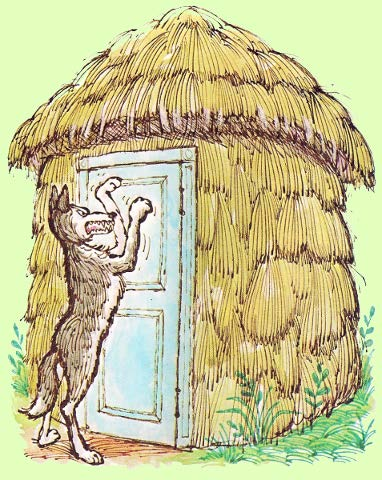
\includegraphics[width=0.9\linewidth]{pic2_20.jpg}
\end{figure}
\end{column}


\begin{column}{.46\linewidth}
\vspace{25pt}
\justifying
\begin{spacing}{1.2}
\rmfamily {\color{Color4}{The next day, the big, bad wolf walked down the road to the first little pig's house of straw. He had one thing on his mind: a nice, juicy pig for his breakfast. He stomped up to the front door, knocked loudly and shouted at the little pig.}}
\end{spacing}
\justifying

\end{column}
\end{columns}
\end{frame}
}


{
\setbeamertemplate{navigation symbols}{\color{black} \insertframenumber/43}
\setcounter{framenumber}{14}
\setbeamertemplate{background canvas}{\color{Color1}\rule{0.48\paperwidth}{\paperheight}\color{Color2}\rule{0.52\paperwidth}{\paperheight}}
\setbeamertemplate{frametitle}[default][right]
\begin{frame}{{\color{white}Emphasize key ideas}}
\begin{columns}
\begin{column}{.5\linewidth}
\begin{spacing}{1.5}
\begin{center}
\textbf{Good}
\end{center}
\begin{enumerate}[\color{black}$\bullet$]
\item Split content into bullet points
\item Use different colors/font styles
\item Add spacing
\end{enumerate}
\end{spacing}
\end{column}

\begin{column}{.55\linewidth}
\begin{spacing}{1.5}
\begin{center}
\textbf{Bad}
\end{center}	
\begin{enumerate}[\color{black}$\bullet$]
\item Write whole sentences
\item Use too many colors/frot styles
\item Have more than 4-6 bullets points
\end{enumerate}
\end{spacing}
\end{column}
\end{columns}
\end{frame}
}


\setbeamercolor{background canvas}{bg=black}
\setbeamertemplate{navigation symbols}{\color{white} \insertframenumber/43}
\setcounter{framenumber}{20}
\begin{frame}{{\color{white}\hspace{164pt}The spy and the villain}}
\begin{columns}

\begin{column}{.35\linewidth}
\begin{figure}[h]

\includegraphics[width=0.9\linewidth]{pic10_21_1.jpg}
\end{figure}
\end{column}
		
\begin{column}{.3\linewidth}
\begin{figure}[h]
\vspace{-30pt}
\includegraphics<3,4>[width=0.95\linewidth]{pic10_21_2.png}
\end{figure}
\end{column}
		
\begin{column}{.35\linewidth}
\begin{figure}[h]
\includegraphics<2,3>[width=0.9\linewidth]{pic10_21_3.jpg}
\includegraphics<4>[width=0.9\linewidth]{pic10_21_4.jpg}
\end{figure}
\end{column}

\end{columns}
\end{frame}
\end{document}
